\Needspace{0.70\textheight}
\section{模型准备}
\label{sec:model-preparation}

\subsection{控制方程}

热风首先与药材表面交换热量和水分，内部状态再通过热传导与扩散发生变化。以圆柱中心轴为轴线，记径向距离为 $r$、时间为 $t$，温度与干基含水率分别为 $T(r,t)$ 和 $C(r,t)$。以下建立固定区域、忽略端部影响时的径向基础模型；其具体适用范围在各问中说明。

图~\ref{fig:cylinder-shell} 给出了药材截面、薄壳微元及表面交换方向。取半径从 $r$ 到 $r+\mathrm{d}r$、长度为 $L$ 的同轴薄壳，建立径向能量守恒关系。图中颜色用于示意升温和失水后的径向差异。

\begin{figure}[H]
  \centering
  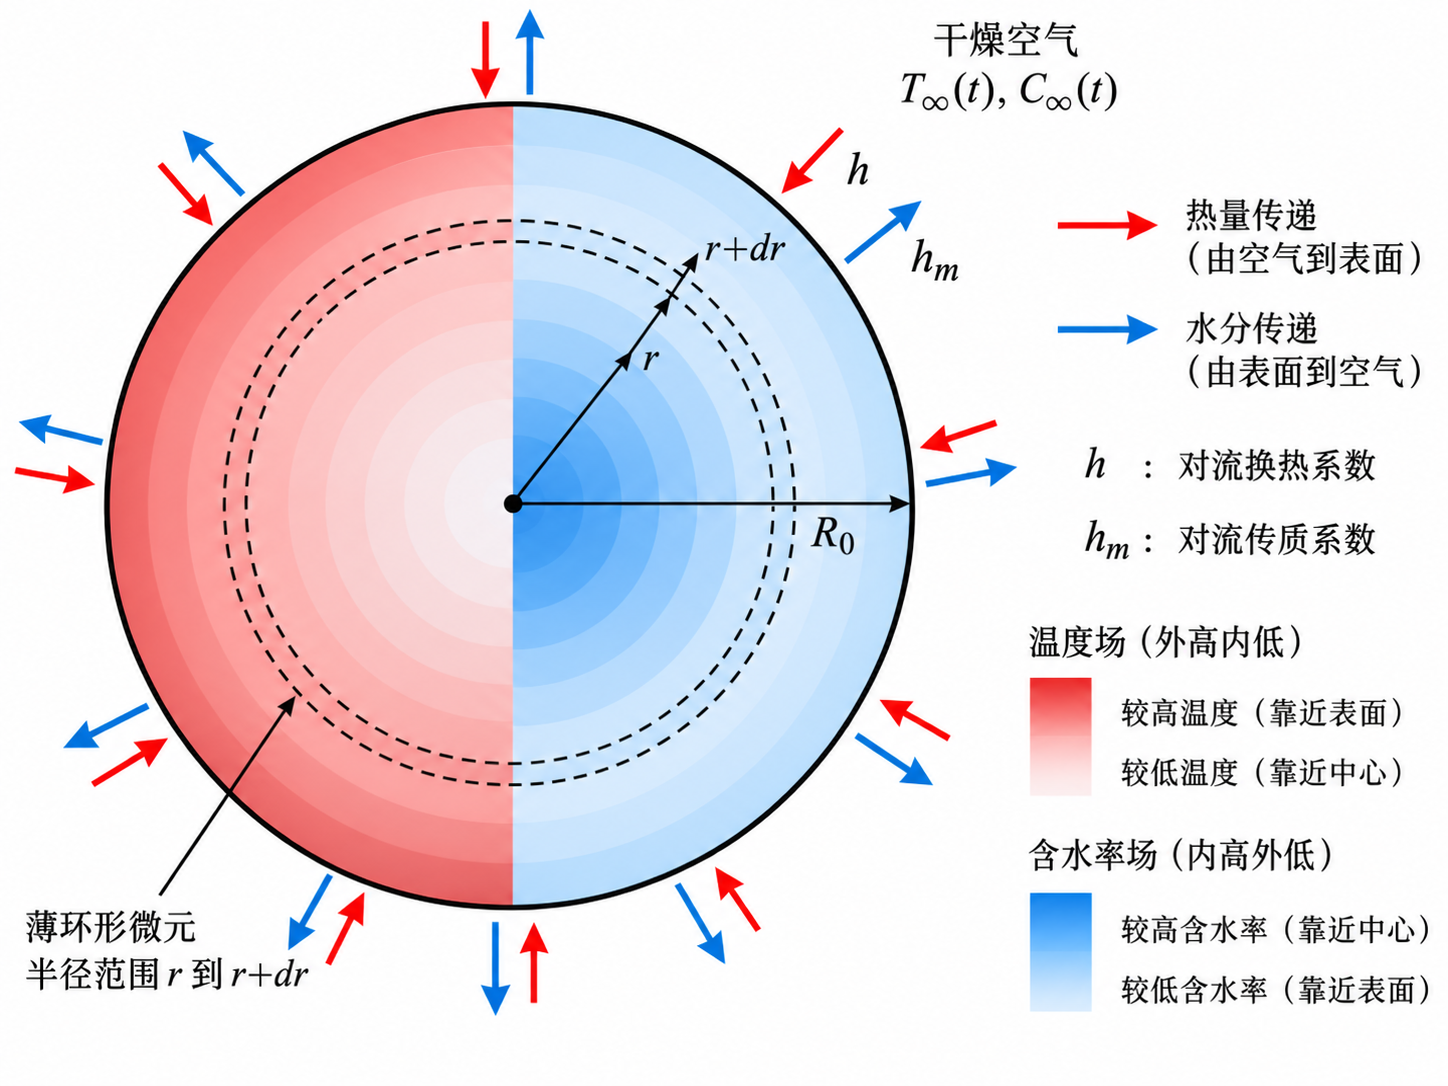
\includegraphics[width=0.90\textwidth]{figures/cylinder_heat_transfer.png}
  \caption{圆柱药材的径向传递及薄壳微元}
  \label{fig:cylinder-shell}
\end{figure}

\noindent\textbf{（1）热传导方程。}根据傅里叶定律，沿半径增大方向通过圆柱面的热流率为

\[
\mathrm{heat}(r,t)
=-2\pi rLk\frac{\partial T}{\partial r}.
\]

取厚度为 $\mathrm{d}r$ 的同轴薄壳，由\textbf{能量守恒}，有

\[
\rho c_p\,2\pi rL\,\mathrm{d}r
\frac{\partial T}{\partial t}
=-\frac{\partial\mathrm{heat}}{\partial r}\,\mathrm{d}r.
\]

代入热流关系并约去公因子，得到圆柱坐标下的一维非稳态热传导方程：

\begin{equation}
\rho c_p\frac{\partial T}{\partial t}
=\frac{1}{r}\frac{\partial}{\partial r}
\left(rk\frac{\partial T}{\partial r}\right),
\qquad 0<r<R_0.
\label{eq:prep-heat}
\end{equation}

式中，$\rho$、$c_p$ 和 $k$ 分别为密度、比热容与导热系数。

\noindent\textbf{（2）水分扩散方程。}将题目所给干基含水率 $C$ 作为有效扩散变量，直接采用圆柱坐标下的 Fick 第二定律：

\begin{equation}
\frac{\partial C}{\partial t}
=\frac{1}{r}\frac{\partial}{\partial r}
\left(rD\frac{\partial C}{\partial r}\right).
\label{eq:prep-moisture}
\end{equation}

$D$ 为有效扩散系数。式~\eqref{eq:prep-heat} 和式~\eqref{eq:prep-moisture} 均\textbf{将物性系数保留在空间微分算子内部}，以便在后续小问中引入状态相关物性；收缩区域还需结合物料运动和区域变化调整输运方程。

\subsection{定解条件}

设初始温度与含水率分别为 $T_0$、$C_0$。均匀初始状态与圆心对称条件写为

\begin{equation}
\left\{
\begin{aligned}
T(r,0)&=T_0,& C(r,0)&=C_0,\\
\left.\frac{\partial T}{\partial r}\right|_{r=0}&=0,
&
\left.\frac{\partial C}{\partial r}\right|_{r=0}&=0.
\end{aligned}
\right.
\label{eq:prep-initial-center}
\end{equation}

记表面状态为 $T_s(t)=T(R_0,t)$、$C_s(t)=C(R_0,t)$，烘房环境量为 $T_\infty(t)$、$C_\infty(t)$。采用对流换热与传质条件：

\begin{equation}
\left\{
\begin{aligned}
-k\left.\frac{\partial T}{\partial r}\right|_{r=R_0}
&=h\left[T_s(t)-T_\infty(t)\right],\\
-D(C_s,T_s)\left.\frac{\partial C}{\partial r}\right|_{r=R_0}
&=h_m\left[C_s(t)-C_\infty(t)\right].
\end{aligned}
\right.
\label{eq:prep-surface}
\end{equation}

其中 $h$、$h_m$ 分别为对流换热和传质系数；若本问的 $D$ 仅与 $C$ 有关，则取 $D(C_s)$。具体物性、环境边界及区域变化在各小问中确定。

\subsection{模型应用}

上述方程构成各问的共同基础。\textbf{第一问}在固定半径、常热物性下计算预热阶段；\textbf{第二问}引入状态相关物性，按本问条件计算全过程，并在阶段切换时延续内部状态；\textbf{第三问}利用第二问的状态演化判定首次全部达标时刻；\textbf{第四问}进一步引入尺寸收缩，调整输运方程、计算区域和表面条件。各问继承同一方程框架，具体物性与区域条件分别确定。
